\newpage
\subsection{Sensitivity to outdoor environment change}
\subsubsection{Effect of noise}
The result in fig. \ref{fig:4mic1srcInd} is applicable only in ideal conditions (zero noise, no reflections and perfectly planar propagation). The localization result for noisy conditions is depicted in fig. \ref{fig:4mic1srcNoisy}. As expected, the performance deteriorates as the SNR drops. 
\begin{figure}[H]
\begin{subfigure}[b]{0.96\textwidth}
    \centering
    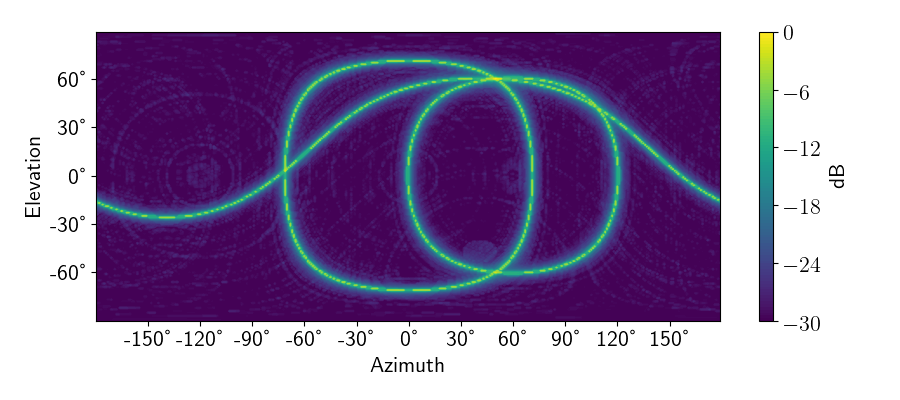
\includegraphics[width=0.8\textwidth]{Figures/Ind4mic1srcRes20.png}
\end{subfigure}
\vskip \baselineskip
\begin{subfigure}[b]{0.96\textwidth}
    \centering
    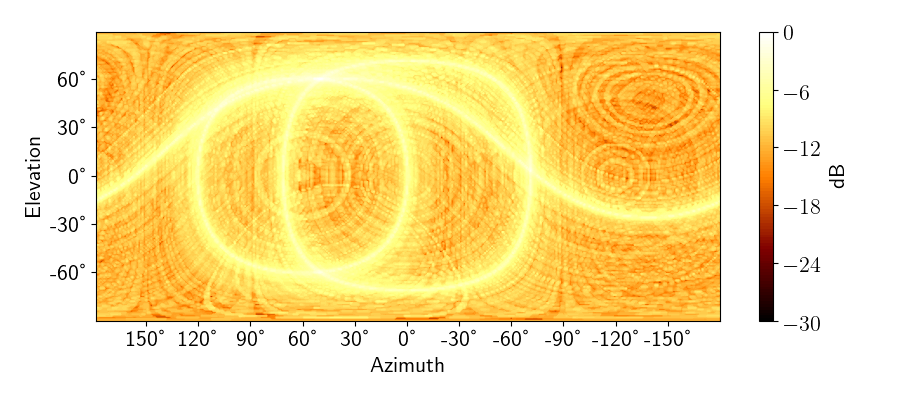
\includegraphics[width=0.8\textwidth]{Figures/Ind4mic1srcRes0.png}
\end{subfigure}
\vskip \baselineskip
\begin{subfigure}[b]{0.96\textwidth}
    \centering
    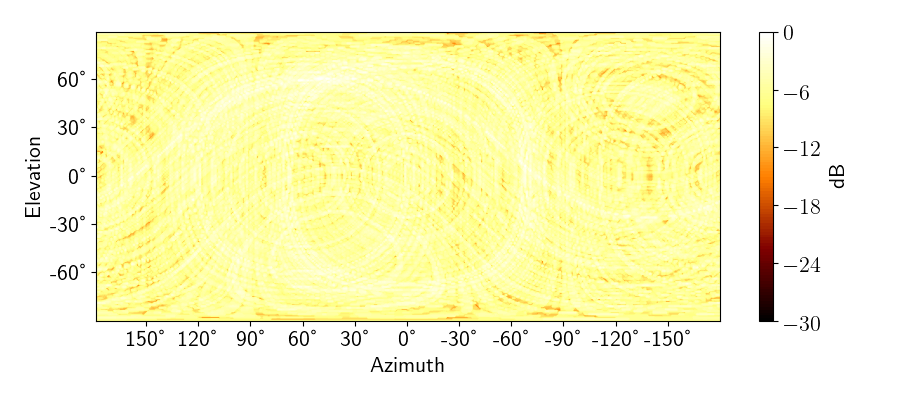
\includegraphics[width=0.8\textwidth]{Figures/Ind4mic1srcResNeg10.png}
\end{subfigure}
\caption{Figures depict from top-to-bottom SRP-PHAT localization results with SNR = 20dB, SNR = 0dB, SNR = -10dB}
\label{fig:4mic1srcNoisy}
\end{figure}
\newpage
\subsubsection{Effect of temperature}
Temperature affects the speed of sound and thus affects the delay time between the microphone pairs. During measurement, if it is assumed to be room temperature, this could lead to errors in the localization results. Fig.\ref{fig:4mic1srcTemp} depicts the effect of temperature on localization results, where wave files received by the tetrahedral microphone array at temperatures of $0\degree C$, $20\degree C$ and $-40\degree C$ are simulated. Then the localization is run assuming the speed of sound to be 343m/sec in every case. The figure shows zoomed in results around the source location. As can be seen in the figure, an error in recording temperature has the effect of `de-focusing' the main peak.
\begin{figure}[H]
    \centering
    \begin{subfigure}[b]{0.96\textwidth}
    \centering
    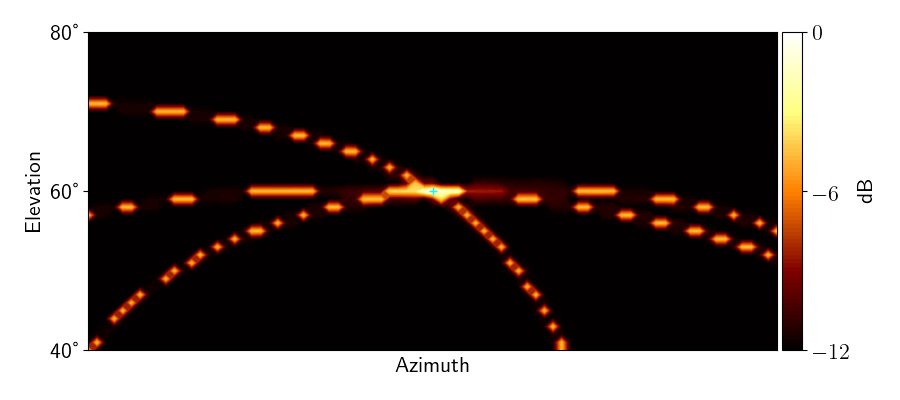
\includegraphics[width=0.8\textwidth]{Figures/Ind4mic1srcSum20deg.png}
\end{subfigure}
\vskip \baselineskip
\begin{subfigure}[b]{0.96\textwidth}
    \centering
    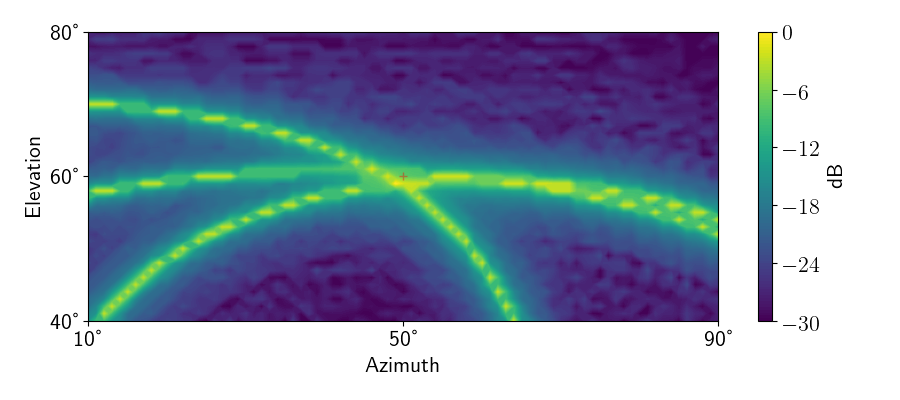
\includegraphics[width=0.8\textwidth]{Figures/Ind4mic1srcSum0deg.png}
\end{subfigure}
\vskip \baselineskip
\begin{subfigure}[b]{0.96\textwidth}
    \centering
    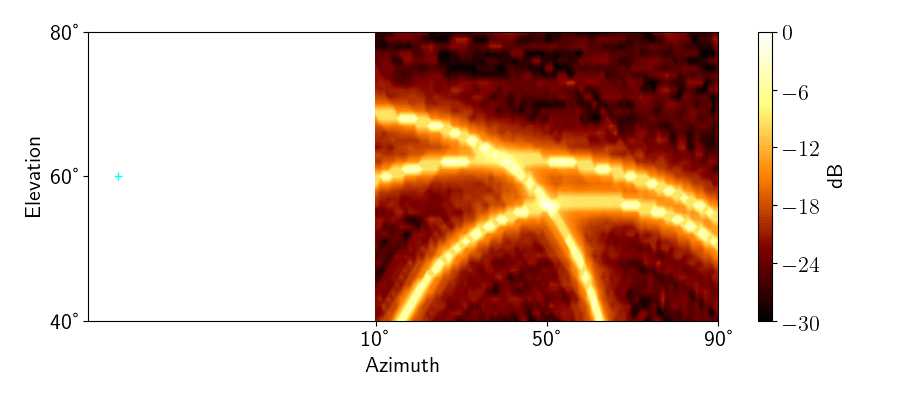
\includegraphics[width=0.8\textwidth]{Figures/Ind4mic1srcSumNeg40deg.png}
\end{subfigure}
\caption{Figures depict from top-to-bottom SRP-PHAT localization results with at temperatures of $20\degree C$, $0\degree C$ and $-40\degree C$.}
\label{fig:4mic1srcTemp}
\end{figure}
\subsubsection{Effect of wind}
Wind speed effects the speed of sound in the direction of propagation. Delays between different array pairs would be affected depending on where the SRP search is looking and from what direction the wind is blowing. If wind blows perpendicular to the direction of propagation of the sound from the source, then it does not affect the localization. Fig.\ref{fig:4mic2srcWind} depicts the effect of wind on localization results at wind of 10$m/s$ blowing at $90\degree$, $45\degree$ and $180\degree$ to a source at ($50\degree$,$60\degree$) without any wind correction. It can be seen that when wind blows at $90\degree$, it does not affect the localization results. The magnitude of error when wind blows non-perpendicular to the sound propagation direction depends on the wind speed and the degree of alignment with the wind direction.
\begin{figure}[H]
    \centering
    \begin{subfigure}[b]{0.96\textwidth}
    \centering
    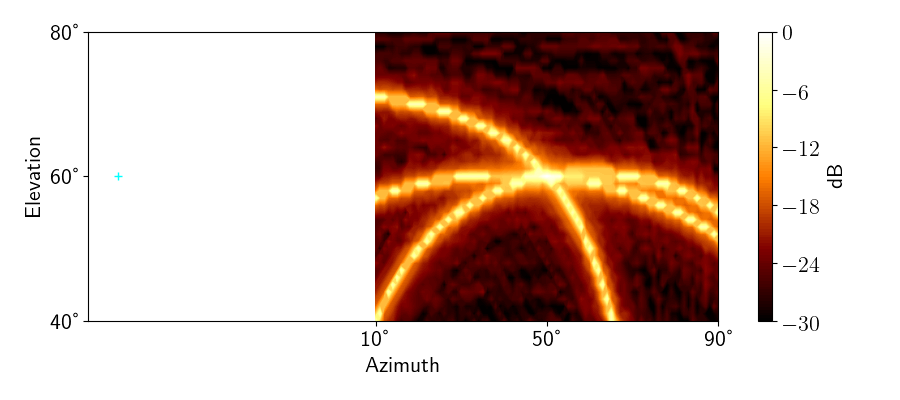
\includegraphics[width=0.8\textwidth]{Figures/4mic1srcWind90.png}
\end{subfigure}
\vskip \baselineskip
\begin{subfigure}[b]{0.96\textwidth}
    \centering
    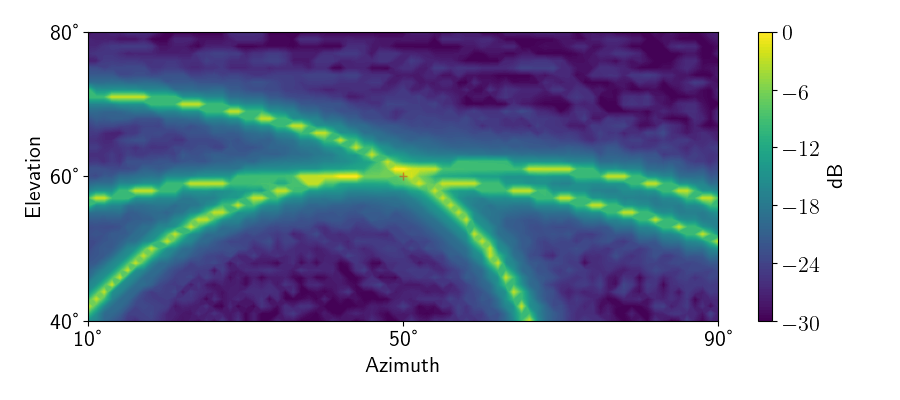
\includegraphics[width=0.8\textwidth]{Figures/4mic1srcWind45.png}
\end{subfigure}
\vskip \baselineskip
\begin{subfigure}[b]{0.96\textwidth}
    \centering
    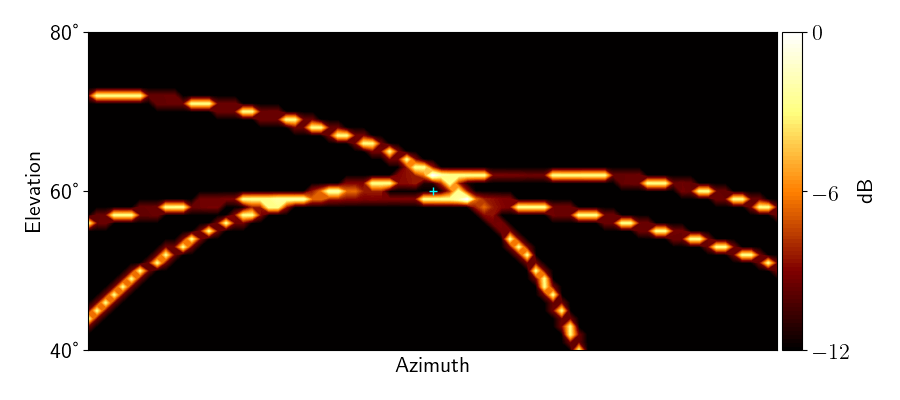
\includegraphics[width=0.8\textwidth]{Figures/4mic1srcWind45Fast.png}
\end{subfigure}
\caption{Figures depict from top-to-bottom SRP-PHAT localization results with wind of $10 m/sec$ blowing $90\degree$, $10 m/sec$ blowing $45\degree$ and $30 m/sec$ blowing $45\degree$ to the source sound propagation direction.}
\label{fig:4mic2srcWind}
\end{figure}
\subsubsection{Effect of ground reflections}
Sound received from a far-field sound source consists of the plane wave and the spherical wave component (Eq. \ref{Eq:GroundWave}). The spherical wave component creates a horizontal ground wave with the ground and quickly attenuates with distance. The plane wave creates a reflected wave with ground (image source) whose magnitude depends on the acoustic reflection coefficient of the ground material. Rudimentary simulations for a source located at $(\theta,\phi)$ can be made assuming image sound source located at $(\theta,-\phi)$. Fig. \ref{fig:4mic1srcRef} shows the localization results with source at ($50\degree$,$60\degree$) for different ground reflection coefficients. The microphone pairs in the tetrahedral array that are parallel to the ground locate both the source and the image on the same cone. This causes the image to be localized at a higher level than it actually is.
\begin{figure}[H]
    \centering
    \begin{subfigure}[b]{0.96\textwidth}
    \centering
    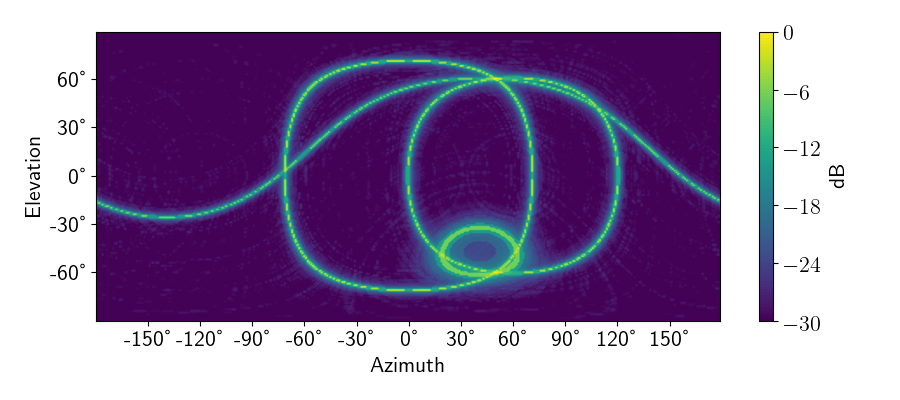
\includegraphics[width=0.8\textwidth]{Figures/4mic1srcRef100.png}
\end{subfigure}
\vskip \baselineskip
\begin{subfigure}[b]{0.96\textwidth}
    \centering
    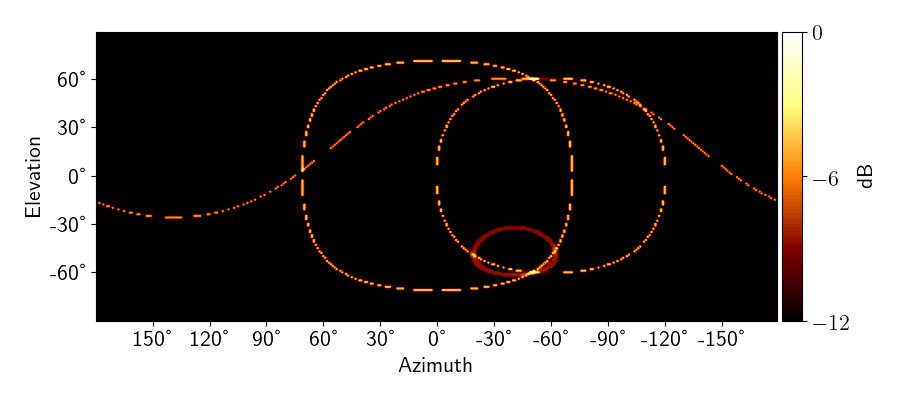
\includegraphics[width=0.8\textwidth]{Figures/4mic1srcRef60.png}
\end{subfigure}
\vskip \baselineskip
\begin{subfigure}[b]{0.96\textwidth}
    \centering
    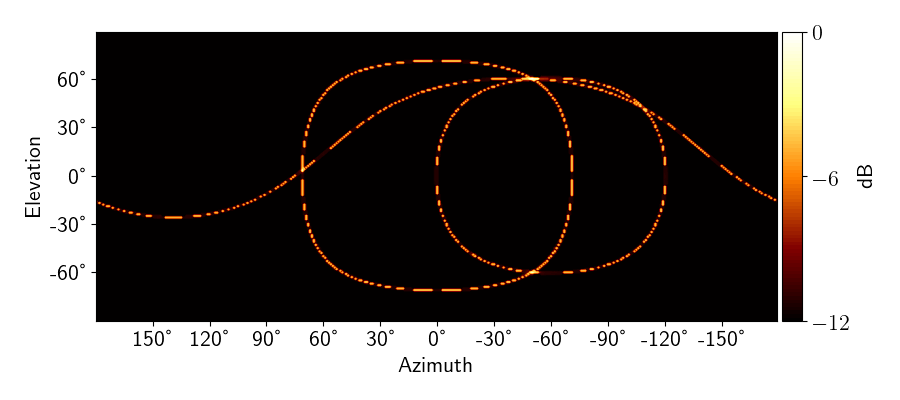
\includegraphics[width=0.8\textwidth]{Figures/4mic1srcRef10.png}
\end{subfigure}
    \caption{Figures depict from top-to-bottom SRP-PHAT localization results with ground reflection coefficients (R) of 1, 0.6 and 0.1. Even though the image source should get significantly weaker for R=0.1, it does not as it is supported by the localization cones from the real source.}
    \label{fig:4mic1srcRef}
\end{figure}